\documentclass[11pt]{book}

\usepackage[utf8]{inputenc}
\usepackage[T1]{fontenc}
\usepackage{amsmath,amssymb,mathtools}
\usepackage{geometry}
\usepackage{tikz}
\usepackage{pgfplots}
\pgfplotsset{compat=1.18}
\geometry{margin=1.15in}

\newcommand{\dd}{\mathrm{d}}

\begin{document}

\chapter[Moving Chains and Ropes]{Moving Chains and Ropes: How the Limit You Take Is the Physics You Get}
\label{chap:chains}

\section{A deceptively simple object}

A chain, mechanically speaking, is about as simple an object as one can write down: a sequence of point masses joined by rigid, massless, frictionlessly-hinged links. A rope is the same idea pushed to a continuum. Every undergraduate meets both within the first month of a mechanics course, usually as a warm-up before the ``real'' problems begin. And yet almost every genuinely dynamical question one can ask about a moving chain or rope --- how it falls, how it whips, how it hangs, how it climbs out of its own container --- turns out to have more than one mathematically defensible answer. The reason is always the same: getting from the discrete picture to a usable equation of motion requires taking something to a limit, and there is more than one limit available. The number of links can be sent to infinity; the length of each link can be sent to zero; the stiffness of the joints can be sent to zero; the mass per unit length can be sent to zero at one end and not the other; the time over which a link joins the moving part of the chain can be sent to zero. These limits are not interchangeable, and taking one instead of another does not merely change the accuracy of an approximation --- it changes which piece of physics you are describing.

This chapter works through four classical problems in which exactly this happens: a hanging rope (statics), a falling chain (dynamics with an unresolved question of energy loss), a self-siphoning ``chain fountain'' (dynamics in which the naive continuum limit throws away a real effect), and a cracking whip (dynamics in which a formally singular limit is nearly realized in the real world). In each case the underlying object --- an inextensible, one-dimensional distribution of mass --- is the same. What differs is a single physical assumption about how that object is loaded, or how it is coupled to whatever it rests on, or how its mass is distributed along its length. The ideal-world equations, written down in the abstract, routinely fail to decide between the available limits on their own; deciding between them is an empirical matter, imported from observation of the actual rope or chain in front of you. That is the sense in which this is a chapter about limits producing physics, rather than merely approximating it.

\section{One family of models, many limits}
\label{sec:family}

Start from the discrete chain: $N$ point masses of mass $m = \lambda \ell$, joined by massless rigid rods of length $\ell$ that are free to pivot at each joint, so that no energy is stored in bending. Writing $\vec r_i(t)$ for the position of the $i$-th mass, the Lagrangian is
\[
L = \sum_{i=1}^{N}\left[\tfrac12 m\, \dot{\vec r}_i^{\,2} - m g y_i\right], \qquad |\vec r_{i+1}-\vec r_i| = \ell \ \ (i=1,\dots,N-1),
\]
the constraints being enforced by Lagrange multipliers that are, physically, the link tensions.

The continuum limit sends $N\to\infty$ and $\ell\to 0$ while holding the linear mass density $\lambda = m/\ell$ and the total length $L = N\ell$ fixed. The position field becomes $\vec r(s,t)$ with $s\in[0,L]$ an arc-length label, and the rigid-link constraint becomes the inextensibility condition $|\partial_s \vec r| = 1$. This continuum object --- massive, perfectly flexible, and inextensible --- is what every mechanics textbook means by ``an ideal chain'' or ``an ideal rope,'' and it is worth being honest about what has been assumed along the way. Perfect flexibility is inherited directly from the discrete picture: because the point masses store no bending energy, neither does their continuum limit. Inextensibility is the statement that the rope's own elastic modulus has effectively been sent to infinity. Neither assumption is free, and \S\ref{sec:fountain} shows a case where discarding the first one \emph{too} readily throws away a real, macroscopically visible force.

A second family of limits concerns how a disturbance travels along the rope once it is under tension. Linearizing the transverse motion of a taut rope with tension profile $T(s)$ and density $\lambda(s)$ gives the wave equation
\begin{equation}
\lambda(s)\,\frac{\partial^2 y}{\partial t^2} = \frac{\partial}{\partial s}\!\left(T(s)\,\frac{\partial y}{\partial s}\right), \qquad c(s) = \sqrt{T(s)/\lambda(s)}.
\label{eq:wave}
\end{equation}
Two more limits sit inside this one equation. If $T/\lambda \to \infty$, disturbances propagate instantaneously: every point of the rope must move together, and the flexible continuum has degenerated into a kinematic constraint --- a rigid rod in everything but name. If $T/\lambda \to 0$, the opposite happens: the rope goes slack, propagation grinds to a halt, and a length of rope can develop a sharp fold or kink that a taut rope could never sustain, because there is no restoring tension to iron it out. Both limits will reappear: the second is exactly what allows a chain to turn a sharp corner at all, whether in a falling heap (\S\ref{sec:falling}), a fountain (\S\ref{sec:fountain}), or a cracking whip (\S\ref{sec:whip}), where $\lambda(s)\to 0$ pointwise and $c(s)\to\infty$ at the tip.

\section{Statics: the shape a rope chooses}
\label{sec:statics}

Before setting anything in motion, it is worth seeing the limit-dependence at work in the simplest possible setting: a rope hanging at rest. Let $H$ denote the (constant) horizontal component of tension along the rope, and let the load per unit length be $q$, whatever it is physically per unit of. Vertical equilibrium of an element gives $\dd(Hy') = q$, and with $y'=\dd y/\dd x$,
\begin{equation}
H y'' = q.
\label{eq:staticgeneric}
\end{equation}
The entire content of the problem is now in the single question: load $q$ per unit of \emph{what}?

If the rope carries only its own weight, uniformly distributed along its own \emph{arc length} $s$, then $q\,\dd x = \lambda g\,\dd s = \lambda g\sqrt{1+y'^2}\,\dd x$, and \eqref{eq:staticgeneric} becomes
\[
y'' = \frac1a\sqrt{1+y'^2}, \qquad a \equiv \frac{H}{\lambda g}.
\]
Separating and integrating twice, with the origin placed at the lowest point,
\begin{equation}
y(x) = a\left[\cosh\!\left(\frac{x}{a}\right) - 1\right] \qquad \text{(the catenary).}
\label{eq:catenary}
\end{equation}

If instead the load is distributed uniformly along the \emph{horizontal} span --- the situation for a suspension-bridge cable, whose own weight is negligible next to that of the deck it carries through closely spaced vertical hangers --- then $q$ is simply a constant $w$ per unit $x$, and \eqref{eq:staticgeneric} integrates at once to
\begin{equation}
y(x) = \frac{w}{2H}x^2 \qquad \text{(the parabola).}
\label{eq:parabola}
\end{equation}

Equations \eqref{eq:catenary} and \eqref{eq:parabola} are not two approximations to the same curve; they are exact solutions of the same static equilibrium condition \eqref{eq:staticgeneric}, differing only in a single real-world fact about how the rope is loaded. Galileo famously guessed the parabola for the hanging-chain problem and was corrected only in 1691, when Leibniz, Huygens, and Johann Bernoulli independently solved the true self-weight problem in response to a challenge posed by Jacob Bernoulli --- historically the first clean demonstration that ``hangs under its own weight'' and ``supports a uniformly spread load'' are different problems with different exact answers, not the same problem solved to different orders of approximation.

They are, however, connected by a limit of their own. For small sag, $|x/a|\ll 1$, expanding \eqref{eq:catenary} gives $y \approx x^2/(2a)$, which is \eqref{eq:parabola} with $w\to \lambda g$. This is exactly the small-sag limit in which arc length and horizontal distance stop being distinguishable ($\dd s\approx \dd x$), so a load spread uniformly in $s$ becomes indistinguishable from one spread uniformly in $x$. A gently sagging catenary and a true parabola are, to this order, the same curve; a deeply sagging one is not. Figure~\ref{fig:catenary} shows both curves for a chain hung with $a=2$, alongside the leading-order parabola that agrees with it only near the bottom.

\begin{figure}[h]
\centering
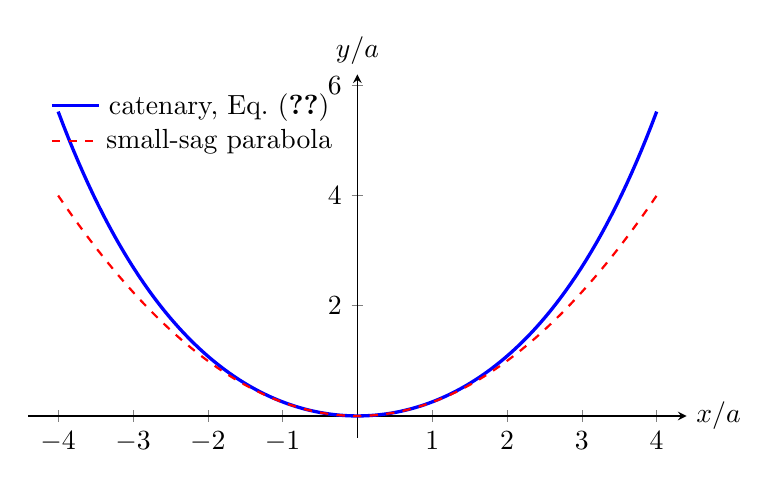
\begin{tikzpicture}
\begin{axis}[
  width=0.82\textwidth, height=6.2cm,
  axis lines=middle,
  xlabel={$x/a$}, ylabel={$y/a$},
  xlabel style={anchor=west}, ylabel style={anchor=south},
  domain=-4:4, samples=120,
  ymin=-0.4, ymax=6.2, xmin=-4.4, xmax=4.4,
  legend style={at={(0.02,0.98)}, anchor=north west, draw=none, fill=none},
]
\addplot[very thick, blue] {exp(x/2)+exp(-x/2)-2};
\addlegendentry{catenary, Eq.~\eqref{eq:catenary}}
\addplot[thick, red, dashed] {x^2/4};
\addlegendentry{small-sag parabola}
\end{axis}
\end{tikzpicture}
\caption{The true hanging shape (catenary) and the parabola that osculates it at the vertex. The two coincide for small sag and diverge visibly once $|x|\gtrsim a$: the same equilibrium equation \eqref{eq:staticgeneric}, closed with two different loading laws, produces two genuinely different curves.}
\label{fig:catenary}
\end{figure}

\section{Dynamics I: the falling chain and the problem of closure}
\label{sec:falling}

Statics leaves the closure of \eqref{eq:staticgeneric} to an explicit modeling choice about the loading law, stated up front. Dynamics is less polite: it is entirely possible to write down what looks like a single, fully specified ``ideal chain'' problem and discover only afterward that the equations of motion do not follow from it uniquely.

The oldest and best-studied example is the chain falling through a hole in a table, first posed by Arthur Cayley in 1857. A chain of linear density $\lambda$ lies coiled in a loose heap on a frictionless table, with one end dangling through a small hole. Let $y(t)$ be the length already hanging below the table, moving as a unit with speed $v=\dot y$; the heap itself sits undisturbed until the instant each link is drawn to the hole.

\paragraph{Closure 1: the pickup is dissipative.} The traditional assumption, and the one that appears in essentially every mechanics textbook from Sommerfeld onward, is that a link sitting in the heap feels no force at all until the moment it reaches the hole, at which point it is snapped from rest to speed $v$ as abruptly as a completely inelastic collision. Newton's second law for the momentum of the moving part, with the newly recruited mass entering with zero momentum, reads
\[
\frac{\dd}{\dd t}\big(\lambda y v\big) = \lambda y g \quad\Longrightarrow\quad v^2 + y\ddot y = yg.
\]
Trying a constant-acceleration solution $y=\tfrac12 a t^2$, $v=at$ gives $a^2t^2 + \tfrac12 a^2 t^2 = \tfrac12 agt^2$, so
\begin{equation}
a = \frac{g}{3} \qquad \text{(non-conservative closure).}
\label{eq:g3}
\end{equation}
This is Cayley's original result, and it is manifestly dissipative: kinetic energy is being destroyed at the hole exactly as in a perfectly inelastic collision, a mechanism first analyzed by Lazare Carnot (father of the Carnot of thermodynamics) more than a century before this problem was posed.

\paragraph{Closure 2: the pickup is reversible.} Nothing in the phrase ``ideal, perfectly flexible chain'' actually forces the pickup to be inelastic. If instead one assumes the whole process conserves mechanical energy --- the falling part's kinetic energy exactly accounting for the gravitational energy released, with no loss at the hole --- then, taking the center of mass of the hanging length at depth $y/2$,
\[
\tfrac12 \lambda y v^2 - \tfrac12 \lambda g y^2 = 0 \quad\Longrightarrow\quad v^2 = gy \quad\Longrightarrow\quad
\]
\begin{equation}
a = \frac{g}{2} \qquad \text{(conservative closure).}
\label{eq:g2}
\end{equation}

Both \eqref{eq:g3} and \eqref{eq:g2} are exact, self-consistent solutions of ``a uniform, frictionless, perfectly flexible chain falls link by link from a resting heap.'' The ideal-world description --- flexible, inextensible, massive curve --- simply does not say which one is correct, because it says nothing about what happens in the infinitesimal neighborhood of the hole, where a link changes in one instant from a member of an undisturbed pile to a member of a moving column. Answering that question requires knowing something about the real chain that is not contained in the word ``ideal'': whether neighboring links can transmit tension through the bend smoothly (favoring energy conservation) or whether each one is genuinely jerked free on its own (favoring dissipation). This is not a settled matter. The $g/3$ answer is the one printed in most textbooks; C.~W.~Wong and K.~Yasui argued in 2006 that Cayley's reasoning is actually wrong even for an idealized chain, on the grounds that it neglects energy handed back by the link \emph{leaving} the stationary heap, and that a properly conservative treatment gives $g/2$. Direct experimental adjudication has proved difficult, because arranging a real heap that behaves cleanly like either idealization is itself hard --- and when careful experiments have been done on real linked chains falling from a heap, Grewal, Johnson, and Ruina (2011) found the chain can speed up \emph{faster still} than either prediction, because a compression wave running back into the heap starts additional links moving before they are individually drawn taut, a mechanism present in neither closure.

\paragraph{A different fold, an opposite answer.} A close cousin of Cayley's problem shows how sensitive the outcome is to exactly how the chain is arranged. Take the same chain, but instead of a heap, fold it so both ends start together at the same height, one end fixed and the other released to fall, so that the falling arm lengthens as the fixed arm's fold descends to feed it (the ``bungee chain'' of Calkin and March, 1989). Here every link remains mechanically continuous with its neighbors right up to and through the fold; there is no sudden edge where an undisturbed pile meets a moving column. Calkin and March measured this directly, on a 1.99~m, 81-link chain, by recording the tension at the fixed support as the chain fell. They found the falling end reaches the floor in about 85\% of the ordinary free-fall time --- it falls \emph{faster} than $g$ --- and that the support tension climbs to roughly 25 times the chain's own weight, far above the $2Mg$ one would expect if the end were simply falling freely and being yanked to a stop. Both facts are consistent only with energy conservation, later confirmed independently by Schagerl and coworkers: the falling arm is being force-fed energy by links that, on rounding the fold, exert a genuine forward push on the arm ahead of them, rather than dissipating their kinetic energy against it. Figure~\ref{fig:heap} sketches the heap version for reference.

\begin{figure}[h]
\centering
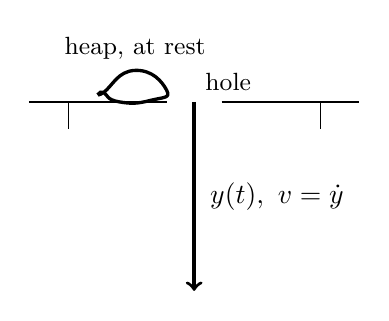
\begin{tikzpicture}[scale=1]
\draw[thick] (-2.1,0) -- (-0.35,0);
\draw[thick] (0.35,0) -- (2.1,0);
\draw (-1.6,0) -- (-1.6,-0.35);
\draw (1.6,0) -- (1.6,-0.35);
\draw[very thick] plot[smooth cycle, tension=1] coordinates {(-1.15,0.12) (-0.75,0.4) (-0.35,0.15) (-0.55,0.02) (-0.95,0.0) (-1.15,0.12)};
\node[above] at (-0.75,0.42) {\small heap, at rest};
\draw[very thick,->] (0,0) -- (0,-2.4);
\node[right] at (0.08,-1.2) {$y(t),\ v=\dot y$};
\node[above right] at (0.02,0.02) {\small hole};
\end{tikzpicture}
\caption{Cayley's falling chain: a heap at rest feeds a moving column through a hole. Whether each link joins the column elastically or inelastically is not fixed by ``ideal chain'' alone, and the two closures give accelerations $g/3$ and $g/2$ respectively.}
\label{fig:heap}
\end{figure}

The lesson of this section is not that one closure is right and the other wrong in general --- it is that the same idealized starting model genuinely underdetermines the dynamics, and the missing information is a real-world fact about the specific chain and the specific fold or heap, not something recoverable from the mathematics of an inextensible curve alone.

\section[Dynamics II: the chain fountain]{Dynamics II: the chain fountain, or when a limit throws away too much}
\label{sec:fountain}

Occasionally a limit is not merely ambiguous but actively wrong, in the sense that it discards a term that turns out to be the whole story. The clearest modern example is the ``chain fountain,'' popularized in a 2013 video by Steve Mould: a chain drawn from a container and allowed to fall over the container's rim rises, before falling, in a self-supporting arc that stands well clear of the rim --- often by tens of centimeters, for a chain draped only a short distance above the floor.

The idealized continuum chain of \S\ref{sec:family} predicts nothing of the kind. Treated as a perfectly flexible, zero-thickness curve, the chain leaving the container has no reason to do anything other than follow the rim, the way a rope follows a frictionless pulley: tension supplies exactly the force needed to bend the chain's path, and there is no mechanism left over to push it higher. Mould's own proposed explanation --- that the falling strand's downward momentum reflects an equal upward momentum into the rising beads --- was shown by John Biggins and Mark Warner (2014) to be untenable on its own terms: if inertia alone were responsible, the chain would momentarily stop at the top of its arc, the way a ball does at the top of a toss, and pile up there. It does not.

Biggins and Warner traced the missing force to exactly the feature the continuum limit had discarded: the finite size of a real link. Modeling the chain as short rigid rods joined by flexible hinges, they noted that when the far end of a link is drawn upward by the chain ahead of it, the pulling force is applied at that end, not at the link's center of mass --- so the link is not just accelerated but torqued, and would rotate its trailing end down into the container floor were the floor not there to stop it. The floor's reaction to this incipient rotation has an upward component beyond ordinary weight-bearing, and this ``kick-off'' is what launches each link above the rim. Set the finite link length to zero, as the naive continuum limit does, and the torque --- and the kick --- vanish identically along with it; the effect is not a small correction sitting on top of the ideal-chain answer, it is a term the ideal-chain limit throws away completely.

The story has not fully closed. Later numerical work by Flekk{\o}y and collaborators (2018) found that rigid links on a smooth container floor do not reproduce a fountain in simulation on their own; a disordered, ``bumpy'' underlying packing of the heap is also needed, and once that disorder is present a fountain appears even for chains with no rod-like rigidity at all, suggesting the geometry of the heap itself, not only the finite length of a link, is doing real work. The full mechanism is, at the time of writing, still being argued over --- which is itself worth remarking on: a century-old-looking toy made of ordinary bead chain does not yet have a universally agreed first-principles explanation. Figure~\ref{fig:fountain} sketches the geometry.

\begin{figure}[h]
\centering
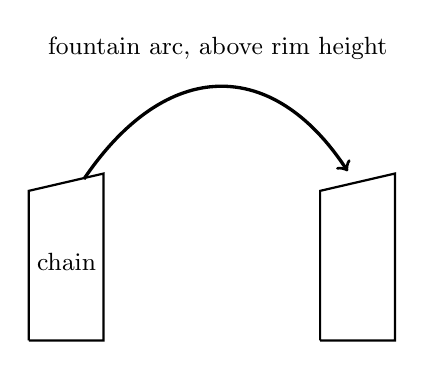
\begin{tikzpicture}
\draw[thick] (-3.1,-1.9) -- (-3.1,0) -- (-2.15,0.22) -- (-2.15,-1.9) -- (-3.1,-1.9);
\node at (-2.62,-0.9) {\small chain};
\draw[very thick,->] (-2.4,0.15) .. controls (-1.35,1.7) and (0.0,1.7) .. (0.95,0.25);
\node[above] at (-0.7,1.55) {\small fountain arc, above rim height};
\draw[thick] (0.6,-1.9) -- (0.6,0) -- (1.55,0.22) -- (1.55,-1.9) -- (0.6,-1.9);
\end{tikzpicture}
\caption{The chain fountain: chain drawn from the left container rises above rim height before falling into the right one. The naive zero-thickness chain model predicts no rise at all.}
\label{fig:fountain}
\end{figure}

\section[Dynamics III: the cracking whip]{Dynamics III: the cracking whip and a singularity nature nearly reaches}
\label{sec:whip}

The wave speed $c(s)=\sqrt{T(s)/\lambda(s)}$ of \eqref{eq:wave} was written for a rope of uniform density; a whip is precisely the case where it is not. A bullwhip tapers continuously from a thick handle to a thin, often braided tip, so $\lambda(s)$ decreases along its length. As an impulse sent down the whip by the wrist travels toward the tip, it moves into a region of ever-smaller $\lambda$, and --- roughly speaking, since the whip is far from a straight taut string and the full treatment must account for its changing shape as it moves --- a shrinking $\lambda$ pushed against a roughly maintained tension pushes the local wave speed up. In the idealized limit of a taper that continues smoothly to $\lambda\to 0$ exactly at the tip, the formal wave speed diverges there, and a disturbance launched from the handle would, in this ideal model, reach the tip in finite time while its speed grows without bound: a genuine finite-time singularity of the idealized equations, not merely a large but finite number.

Early twentieth-century high-speed photography had already shown that a whip's crack really is a small sonic boom: some part of the whip genuinely exceeds the speed of sound in air. What was not settled until Alain Goriely and Tyler McMillen's 2002 analysis was which part, and why. Earlier treatments had proceeded by assuming a particular conserved quantity --- energy along the whip in one approach, momentum in another --- together with an assumed taper shape, and different choices of what to hold fixed gave qualitatively different limiting behavior: the tip speed diverging to infinity in some treatments, approaching a finite constant in others. This is the same phenomenon as the falling-chain closure problem in a different guise: a family of superficially similar idealizations, distinguished only by which conservation law is imposed by hand, yielding different physics. Goriely and McMillen resolved the ambiguity by not assuming a shape at all, instead solving the coupled equations for an inextensible, unshearable, tapering elastic rod self-consistently for its motion and geometry together. Their result: the crack is produced not by the geometric tip itself but by a folded loop that travels down the whip, accelerating as the local radius shrinks beneath it, and it is this loop that first crosses the speed of sound, while the true tip --- moving even faster, by their calculation more than thirty times the initiating handle speed --- is by then riding in the loop's acoustic wake and cannot itself generate a shock.

The whip is thus a case, unlike the chain fountain, in which the naive singular limit is not simply wrong: it correctly predicts that something dramatic happens as $\lambda\to 0$, and a real, physically tapering object gets close enough to that limit to produce an audible, measurable sonic boom, before other effects --- the whip's finite total length, air resistance, and the material's finite tensile strength --- necessarily intervene to prevent the true mathematical divergence from being reached.

\section{Synthesis: five lessons from one Lagrangian}
\label{sec:synthesis}

Every example in this chapter descends from the same starting point: a one-dimensional, inextensible distribution of mass, obtained as the continuum limit of point masses on rigid links. What changed between examples was never the starting Lagrangian; it was which additional limit, or which additional physical assumption standing in for a limit, was imposed to close the problem.

\begin{itemize}
\item In statics, the closure was a choice of loading law --- per unit arc length or per unit horizontal length --- and the two choices are connected by a further, small-sag limit in which they become indistinguishable.
\item In the falling chain, the closure was a choice about the microscopic nature of a pickup event that the continuum model does not itself resolve, and the two available choices give different, both self-consistent, accelerations; a closely related setup (the folded chain) shows the same kind of pickup can sit unambiguously on the conservative side, once the geometry removes the sudden edge between rest and motion.
\item In the chain fountain, the culprit was a limit taken too readily: sending the link length to zero removes a torque, and with it a real force, that has no counterpart once the limit is taken.
\item In the whip, a formally singular limit --- density going to zero at a point --- turned out to be approximately realized by an actual physical object, producing a genuine, audible new phenomenon rather than a runaway approximation error, and doing so in a way that itself depended on which conserved quantity one chose to hold fixed while getting there.
\item Underlying all of them is the stiffness limit of \S\ref{sec:family}: it is precisely because a chain or rope can go locally slack, $T/\lambda\to 0$, that it can fold sharply enough to support a heap, a fountain kick-off, or a whip's traveling loop in the first place; a permanently taut, $T/\lambda\to\infty$ rope could do none of these things.
\end{itemize}

None of this is a criticism of the idealized chain as a model --- it is, after all, precisely what makes each of these problems tractable at all. It is a reminder that an idealization is never self-interpreting. ``Perfectly flexible,'' ``inextensible,'' and ``uniform'' are limits, and every limit has a rate and a direction, decided somewhere outside the mathematics, by the real object the mathematics is standing in for. Chains and ropes are unusually good at making this visible, because the relevant real-world fact is often small enough to seem safely negligible --- the size of a single link, the elasticity of a single joint, the way one particular pile happens to be stacked --- right up until it turns out to be the only thing separating one piece of physics from another.

\section*{Further reading}
\begin{itemize}
\item A.~Cayley, ``On a class of dynamical problems,'' \emph{Proc. Roy. Soc. London} \textbf{8}, 506 (1857).
\item M.~G.~Calkin and R.~H.~March, ``The dynamics of a falling chain: I,'' \emph{Am. J. Phys.} \textbf{57}, 154 (1989); M.~G.~Calkin, ``The dynamics of a falling chain: II,'' \emph{Am. J. Phys.} \textbf{57}, 157 (1989).
\item C.~W.~Wong and K.~Yasui, ``Falling chains,'' \emph{Am. J. Phys.} \textbf{74}, 490 (2006).
\item C.~W.~Wong, S.~H.~Youn, and K.~Yasui, ``The falling chain of Hopkins, Tait, Steele and Cayley,'' \emph{Eur. J. Phys.} \textbf{28}, 385 (2007).
\item A.~Grewal, P.~Johnson, and A.~Ruina, ``A chain that speeds up, rather than slows, due to collisions: how compression can cause tension,'' \emph{Am. J. Phys.} \textbf{79}, 723 (2011).
\item J.~S.~Biggins and M.~Warner, ``Understanding the chain fountain,'' \emph{Proc. R. Soc. A} \textbf{470}, 20130689 (2014).
\item E.~G.~Flekk{\o}y et al., ``Mechanisms of the flying chain fountain,'' \emph{Front. Phys.} \textbf{6}, 84 (2018).
\item A.~Goriely and T.~McMillen, ``Shape of a cracking whip,'' \emph{Phys. Rev. Lett.} \textbf{88}, 244301 (2002).
\item T.~McMillen and A.~Goriely, ``Whip waves,'' \emph{Physica D} \textbf{184}, 192 (2003).
\end{itemize}

\end{document}
